%\documentclass[mathserif,17pt,xcolor=table]{beamer}
\documentclass[mathserif,14pt,xcolor=table]{beamer}

\usepackage {bbm}
\usepackage {textpos}

\definecolor{utorange}{RGB}{203,96,21}
\definecolor{utblack}{RGB}{99,102,106}
\definecolor{utbrown}{RGB}{110,98,89}
\definecolor{utsecbrown}{RGB}{217,200,158}
\definecolor{utsecgreen}{RGB}{208,222,187}
\definecolor{utsecblue}{RGB}{127,169,174}

\mode<presentation>
{
    % \usetheme{Pittsburgh}   
    \usetheme{Boadilla}  
    %\usetheme{Darmstadt}
    \usefonttheme[onlymath]{serif}

    %\AtBeginSection[] {
    %    %\setbeamercolor{subsection in toc}{fg=utblack!50}
    %    \begin{frame}<beamer>
    %    \frametitle{Outline}
    %    \tableofcontents[
    %        currentsection, currentsubsection
    %        %subsectionstyle=show,
%   %         hideothersubsections
    %    ]
    %  \end{frame}
    %}
    \AtBeginSubsection[]
    {
        %\setbeamercolor{subsection in toc}{fg=utblack!50}
        \begin{frame}<beamer>
        \frametitle{Outline}
        \tableofcontents[
            currentsubsection,
            %subsectionstyle=show,
%            hideothersubsections
        ]
      \end{frame}
    }
  

    \setbeamercovered{invisible}
    % get rid of the navigation symbols
    \setbeamertemplate{navigation symbols}{}

    % Color Theme 
    \setbeamercolor{normal text}{bg=white,fg=utblack}
    \setbeamercolor{structure}{fg=utorange}

    \setbeamercolor{alerted text}{fg=red!85!black}

    \setbeamercolor{item projected}{use=item,fg=black,bg=item.fg!35}

    \setbeamercolor*{palette primary}{use=structure,fg=white, bg=utorange}
    \setbeamercolor*{palette secondary}{use=structure,bg=utsecbrown}
    \setbeamercolor*{palette tertiary}{use=structure,bg=utsecgreen}
    \setbeamercolor*{palette quaternary}{use=structure,fg=structure.fg,bg=utsecblue}

    \setbeamercolor*{title}{fg=white, bg=utorange}
    %\setbeamercolor*{frametitle}{fg=white, bg=utblack}
    \setbeamercolor*{frametitle}{fg=white, bg=utorange}
    % \setbeamercolor*{frametitle}{use=structure,fg=utorange, bg=utsecbrown}
    % \setbeamercolor*{framesubtitle}{fg=utbrown, bg=utsecbrown}

    \setbeamercolor*{date in head/foot}{bg=utsecblue,fg=black}
    \setbeamercolor*{block title}{parent=structure,fg=black,bg=utsecgreen}
    \setbeamercolor*{block body}{fg=black,bg=utblack!10}
    \setbeamercolor*{block title alerted}{parent=alerted text,bg=black!15}
    \setbeamercolor*{block title example}{parent=example text,bg=black!15}

    %\setbeamerfont{frametitle}{size=\Huge}
    %\setbeamerfont{framesubtitle}{size=\small}
    \setbeamerfont{title}{shape=\slshape,series=\bfseries}
    \setbeamerfont{subtitle}{shape=\upshape,series=\mdseries}
    \setbeamerfont{block title}{size=\normalsize}
}

%\usepackage[orientation=landscape,size=custom,width=16,height=12,scale=0.6,debug]{beamerposter}
%\usepackage[orientation=landscape,size=custom,width=16,height=9.75,scale=0.5,debug]{beamerposter}
%\usepackage[orientation=landscape,size=custom,width=16,height=9,scale=0.5,debug]{beamerposter}


\makeatletter
\makeatother

\usepackage{kerkis}
\usepackage[T1]{fontenc}
%\usepackage[protrusion=true,expansion=true]{microtype}
\usepackage{amsmath}
\usepackage{epstopdf}
\usepackage{epsfig}
\usepackage{tikz}
\usepackage{listings}             
\usepackage{calc}
\usepackage{ulem}

%\lstset {
%    language=Java,
%    basicstyle=\footnotesize\ttfamily,
%    keywordstyle=\footnotesize\color{blue}\ttfamily,
%}


\lstdefinestyle{highlight}{
    keywordstyle=\color{blue},
    keywordstyle=[2]\color{utorange},
    commentstyle=\color{red},
}
\lstdefinestyle{base}{
    language={Java},
    basicstyle=\color{black!60}\footnotesize\ttfamily,
    keywordstyle=\color{blue!60},
    keywordstyle=[2]\color{utorange!60},
    commentstyle=\color{red!60},
    moredelim=**[is][\only<+>{\color{black}\bfseries\lstset{style=highlight}}]{@}{@},
    keywords=[2]{AutoSynch, waituntil},
}

\lstdefinestyle{tinybase}{
    language={Java},
    basicstyle=\color{black}\tiny\ttfamily,
    keywordstyle=\color{blue},
    keywordstyle=[2]\color{utorange},
    commentstyle=\color{red},
    keywords=[2]{AutoSynch, waituntil},
}

\renewcommand*{\thefootnote}{\fnsymbol{footnote}}

\pgfdeclareimage[height=1.0cm]{utbig}{logos/UTWordmark}
\pgfdeclareimage[height=0.6cm]{ut}{logos/UTWordmark}
% \pgfdeclareimage[height=1.5cm]{sclogo}{logos/SC12}
% \pgfdeclareimage[height=1.0cm]{scsmall}{logos/SC12}


\title[AutoSynch]{AutoSynch}
\subtitle{An Automatic-Signal Monitor \\Based on Predicate Tagging}
%\author[Wei-Lun Hung]{ \underline{Wei-Lun Hung} \and Vijay K.\, Garg}

\author[W.L.\ Hung \& V. K. Garg]{ 
    \texorpdfstring{
        \begin{columns}[T]
            \column{0.40\linewidth}
            \centering
            \underline{Wei-Lun Hung} \\
            \href{mailto:wlhung@utexase.edu}{\footnotesize wlhung@utexas.edu}
            \column{0.40\linewidth}
            \centering
            Vijay K. Garg \\
            \href{mailto:garg@ece.utexas.edu}{\footnotesize garg@ece.utexas.edu}
        \end{columns}
    }
    {Wei-Lun Hung \& Vijay K. Garg}
}


\institute[UT Austin] 
{
    Parallel and Distributed Systems Laboratory \\
    Department of Electrical \& Computer Engineering \\ \mbox{}  \\  
    \pgfuseimage{utbig} 
}
\date[PLDI 2013]
%{\pgfuseimage{sclogo} }

\begin{document}

    \tikzstyle{block} = [rectangle, draw, rounded corners, shade, top color=white, text width=5em,
        bottom color=blue!50!black!20, draw=blue!40!black!60, very thick, 
        text centered, minimum height=4em]
    \tikzstyle{line} = [draw, -latex']
    \tikzstyle{cloud} = [draw, ellipse,top color=white, bottom color=red!20, 
        node distance=2cm, minimum height=2em]


    %\beamertemplateballitem
    \beamertemplatetransparentcoveredhigh
    { 
        \setbeamertemplate{footline}{
            \hbox{%
            \begin{beamercolorbox}[wd=.78\paperwidth,ht=2.25ex,dp=1ex,center]
                {title in head/foot}
            \end{beamercolorbox}

            \begin{beamercolorbox}[wd=.2\paperwidth,ht=2.25ex,dp=1ex,right]{date in head/foot}%
                \usebeamerfont{date in head/foot}\insertshortdate{}\hspace*{2em}
            \end{beamercolorbox}}%
            \vskip0pt%
        } 
        \frame{\titlepage}
    }
    %\addtobeamertemplate{frametitle}{}{%
    %    \begin{textblock*}{100mm}(0.95\textwidth,-0.75cm)
    %  \pgfuseimage{ut}
    %  \end{textblock*}
    %}

\addtocounter{framenumber}{-1}
\setbeamertemplate{footline}
{
  \leavevmode%
    \hbox{%
    %  \begin{beamercolorbox}[wd=.333333\paperwidth,ht=2.25ex,dp=1ex,center]{author in head/foot}%
    %    \usebeamerfont{author in head/foot}\insertshortauthor%~~\beamer@ifempty{\insertshortinstitute}{}{(\insertshortinstitute)}
    %  \end{beamercolorbox}%
    %    \begin{beamercolorbox}[wd=.333333\paperwidth,ht=2.25ex,dp=1ex,center]{title in head/foot}%
    %    \usebeamerfont{title in head/foot}\insertshorttitle
    %    \end{beamercolorbox}%
    \begin{beamercolorbox}[wd=.78\paperwidth,ht=2.25ex,dp=1ex,center]
        {title in head/foot}
    \end{beamercolorbox}

        \begin{beamercolorbox}[wd=.2\paperwidth,ht=2.25ex,dp=1ex,right]{date in head/foot}%
        \usebeamerfont{date in head/foot}\insertshortdate{}\hspace*{2em}
        \insertframenumber{} / \inserttotalframenumber\hspace*{2ex} 
      \end{beamercolorbox}}%
        \vskip0pt%
}


\section{Introduction}

    \begin{frame}<beamer>
        \frametitle{Outline}
        \tableofcontents[
            currentsubsection,
        ]
    \end{frame}
% ------------------------------------------------------------
%\begin{frame}[t]
%    \frametitle{Motivation}
%    \begin{itemize}
%        \item {\bf Concurrent programming} is necessary 
%            %\begin{itemize}
%            %    \item Clock speed wall
%            %    \item Multi-cores are everywhere
%            %\end{itemize}
%    
%        \item Using locks and condition variables to provide {\bf mutual 
%            exclusion} and {\bf synchronization} of parallel threads on shared 
%            memory 
%            \begin{itemize}
%                \item Signal vs. signalAll
%                \item while instead of if
%            \end{itemize}
%        \item {\bf Automatic-signal monitor} can simplify concurrent 
%            programming
%            \begin{itemize}
%                \item No notation of explicit condition variables 
%                \item Allowing gains in productivity of the programmer as well
%                    as gain in performance of the system
%            \end{itemize}
%    \end{itemize}
%\end{frame}

%\subsection{A Motivating Example}
\begin{frame}[fragile]
    \frametitle{Bounded Buffer}
    \begin{lstlisting}[style=base]
        public class BoundedBuffer {
          Object[] buff;
          int putPtr, takePtr, count;
          @// for mutual exclusion and synchronization 
          Lock mutex = new ReentrantLock();
          Condition full = mutex.newCondition();
          Condition empty = mutex.newCondition();@
          public BoundedBuffer(int n) {
            buff = new Object[n];
            putPtr = takePtr = count = 0;
          }
        }
    \end{lstlisting}
\end{frame}

%\begin{frame}[fragile]
%    \frametitle{A Bounded Buffer}
%    \begin{lstlisting}[style=base]
%          public void put(Object item) {
%            @// lock before operations
%            mutex.lock();
%            // wait if the buffer is full
%            while (count == buff.length) {
%              full.await();
%            }@
%            buff[putPtr++] = item;
%            putPtr %= buff.length;
%            count++;
%            @// signal other threads when the buffer 
%            // is no longer empty
%            if (count == 1) {
%              empty.signalAll();
%            }
%            // unlock after operations
%            mutex.unlock();@
%          }
%    \end{lstlisting}
%\end{frame}

%\begin{frame}[fragile]
%    \frametitle{A Bounded Buffer}
%    \begin{lstlisting}[style=base]
%          public void put(Object item) {
%            mutex.lock();
%            @// Need loop to check the intended condition
%            // if (count == buff.length) {
%            while (count == buff.length) {@
%              full.await();
%            }
%            buff[putPtr++] = item;
%            putPtr %= buff.length;
%            count++;
%            if (count == 1) {
%              @// Use wrong waiting notification
%              // empty.signal() 
%              empty.signalAll();@
%            }
%            mutex.unlock();
%          }
%    \end{lstlisting}
%\end{frame}


\begin{frame}[fragile]
    \frametitle{Bounded Buffer}
    \begin{lstlisting}[style=base]
          public Object take() {
            @// lock before operations
            mutex.lock();
            // wait if the buffer is empty 
            while (count == 0) {
              empty.await();
            }@
            Object ret = buff[takePtr++];
            takePtr %= buff.length;
            count--;
            @// signal other threads when the buffer 
            // is no longer full
            if (count == buff.length - 1) {
              full.signalAll();
            }
            // unlock after operations
            mutex.unlock();@
          } 
    \end{lstlisting}
\end{frame}

\begin{frame}[fragile]
    \frametitle{Bounded Buffer: Common Bugs}
    \begin{lstlisting}[style=base]
          public Object take() {
            mutex.lock();
            if (count == 0) {
              empty.await();
            }
            Object ret = buff[takePtr++];
            takePtr %= buff.length;
            count--;
            if (count == buff.length - 1) {
              full.signal();
            }
            mutex.unlock();
          }
    \end{lstlisting}
\end{frame}

\begin{frame}[fragile]
    \frametitle{Bounded Buffer: Common Bugs}
    \begin{lstlisting}[style=base, escapechar=!]
          public Object take() {
            mutex.lock();
            !{\bf\footnotesize\ttfamily\color{blue}{\color{red}\sout{if}} while}! (count == 0) {
              empty.await();
            }
            Object ret = buff[takePtr++];
            takePtr %= buff.length;
            count--;
            if (count == buff.length - 1) {
              full.signal();
            }
            mutex.unlock();
          }
    \end{lstlisting}
\end{frame}

\begin{frame}[fragile]
    \frametitle{Bounded Buffer: Common Bugs}
    \begin{lstlisting}[style=base, escapechar=!]
          public Object take() {
            mutex.lock();
            while (count == 0) {
              empty.await();
            }
            Object ret = buff[takePtr++];
            takePtr %= buff.length;
            count--;
            if (count == buff.length - 1) {
              !{\bf\footnotesize\ttfamily\color{black}{\color{red}\sout{
              full.signal()}} full.signalAll()}!;
            }
            mutex.unlock();
          }
    \end{lstlisting}
\end{frame}

\begin{frame}[fragile]
    \frametitle{AutoSynch Bounded Buffer}
    \begin{lstlisting}[style=base]
        public @AutoSynch@ class BoundedBuffer {
          Object[] buff;
          int putPtr, takePtr, count;
          public BoundedBuffer(int n) {
            buff = new Object[n];
            putPtr = takePtr = count = 0 ;
          }
        }
    \end{lstlisting}
\end{frame}

%\begin{frame}[fragile]
%    \frametitle{An AutoSynch Bounded Buffer}
%    \begin{lstlisting}[style=base]
%          public void put(Object item) {
%            @waituntil (count < buff.length);@
%            buff[putPtr++] = item;
%            putPtr %= buff.length;
%            count++;
%          }
%    \end{lstlisting}
%\end{frame}

\begin{frame}[fragile]
    \frametitle{AutoSynch Bounded Buffer}
    \begin{lstlisting}[style=base]
          public Object take() {
            @waituntil (count > 0);@
            Object ret = buff[takePtr++];
            takePtr %= buff.length;
            count--;
          }
    \end{lstlisting}
\end{frame}

%\begin{frame}[fragile]
%    \frametitle{Another Bounded Buffer}
%    \only<1> {
%        \lstinputlisting[bb1]{boundedbuffer.tex}
%    }
%    \only<2> {
%        \lstinputlisting[bb2]{boundedbuffer_put.tex}
%    }
%    \only<3> {
%        \lstinputlisting[bb3]{boundedbuffer_take.tex}
%    }
%\end{frame}

%\begin{frame}[t]
%    \frametitle{Example}
%\end{frame}

\begin{frame}[fragile]
    \frametitle{AutoSynch vs. Explicit Signaling}

    \begin{columns}
        \column{0.45\textwidth}
        \begin{lstlisting}[style=tinybase, gobble=8, numbers=left,
            numbersep=-10pt]
            public AutoSynch class BoundedBuffer {
              Object[] buff;
              int putPtr, takePtr, count;
              public BoundedBuffer(int n) {
                buff = new Object[n];
                putPtr = takePtr = count = 0 ;
              }
              public Object take() {
                waituntil (count > 0);
                Object ret = buff[takePtr++];
                takePtr %= buff.length;
                count--;
              }
            }
        \end{lstlisting}
        \column{0.55\textwidth}
        \begin{lstlisting}[style=tinybase, gobble=8, numbers=left,
            numbersep=-10pt]
            public class BoundedBuffer {
              Object[] buff;
              int putPtr, takePtr, count;
              Lock mutex = new ReentrantLock();
              Condition full = mutex.newCondition();
              Condition empty = mutex.newCondition();
              public BoundedBuffer(int n) {
                buff = new Object[n];
                putPtr = takePtr = count = 0;
              }
              public Object take() {
                mutex.lock();
                while (count == 0) {
                  empty.await();
                }
                Object ret = buff[takePtr++];
                takePtr %= buff.length;
                count--;
                if (count == buff.length - 1) {
                  full.signalAll();
                }
                mutex.unlock();
              }
            }
        \end{lstlisting}
    \end{columns}
\end{frame}

%\begin{frame}
%    \frametitle{Why Explicit Signaling Bad?} 
%    \begin{itemize}
%        \item Code is more complex
%        \item More bugs
%        \item Violating separation of concerns
%    \end{itemize}
%    By analogy with the relationship between garbage collection and manual 
%    memory allocation
%\end{frame}

%\subsection{Challenges and Opportunities}
\begin{frame}
    \frametitle{Related Work} 
    \begin{itemize}
        \item The idea of automatic signaling was suggested 
            by Hoare in [Hoa74], but rejected due to efficiency considerations  
        \item The common belief: automatic signaling is extremely
            inefficient compared to explicit signaling [BFC95][BH05]
    \end{itemize}
\end{frame}

\begin{frame}
    \frametitle{Opportunity}
    The signalAll call
    \begin{itemize}
        \item Introduces redundant context switches
        \item Is required in explicit signaling 
    \end{itemize}
\end{frame}

\begin{frame}
    \frametitle{Parameterized Bounded Buffer}
    \begin{figure}[ht!]
        \centering
        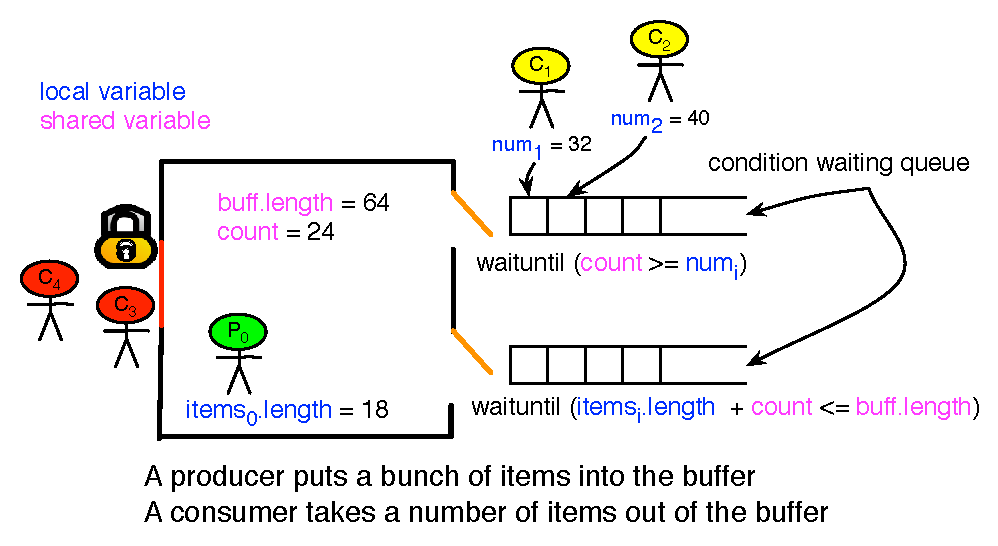
\includegraphics[scale=0.75]{fig/pbb.eps}
        \label{fig:fw}
    \end{figure}
\end{frame}

%\begin{frame}[fragile]
%    \frametitle{A Parameterized Bounded Buffer}
%    \begin{lstlisting}[style=base, gobble=4]
%          public void put(@Object[] items@) {
%            mutex.lock();
%            while (items.length + count > buff.length) {
%              @insufficientSpace.await();@
%            }
%            for (int i = 0; i < items.length; i++) {
%              buff[putPtr++] = items[i];
%              putPtr %= buff.length;
%            }
%            count += items.length;
%            @insufficientItem.signalAll()@;
%            mutex.unlock();
%          }
%    \end{lstlisting}
%\end{frame}

%\begin{frame}[fragile]
%    \frametitle{A Parameterized Bounded Buffer}
%    \begin{lstlisting}[style=base, gobble=4]
%          public Object[] take(@int num@) {
%            mutex.lock();
%            while (count < num) {
%              @insufficientItem.await();@
%            }
%            Object[] ret = new Object[num];
%            for (int i = 0; i < num; i++) {
%              ret[i] = buff[takePtr++];
%              takePtr %= buff.length;
%            }
%            count -= num;
%            @insufficientSpace.signalAll();@
%            mutex.unlock();
%            return ret;
%          }
%    \end{lstlisting}
%\end{frame}

%\begin{frame}[fragile]
%    \frametitle{A Parameterized Bounded Buffer}
%    1 producer randomly puts 1 to 128 items per time \\
%    Every consumer randomly takes 1 to 128 items per time  \\
%    Total 512000 items are put and taken 
%    \begin{columns}[c]
%        \column{0.5\textwidth}
%        \begin{figure}[ht!]
%            \centering
%            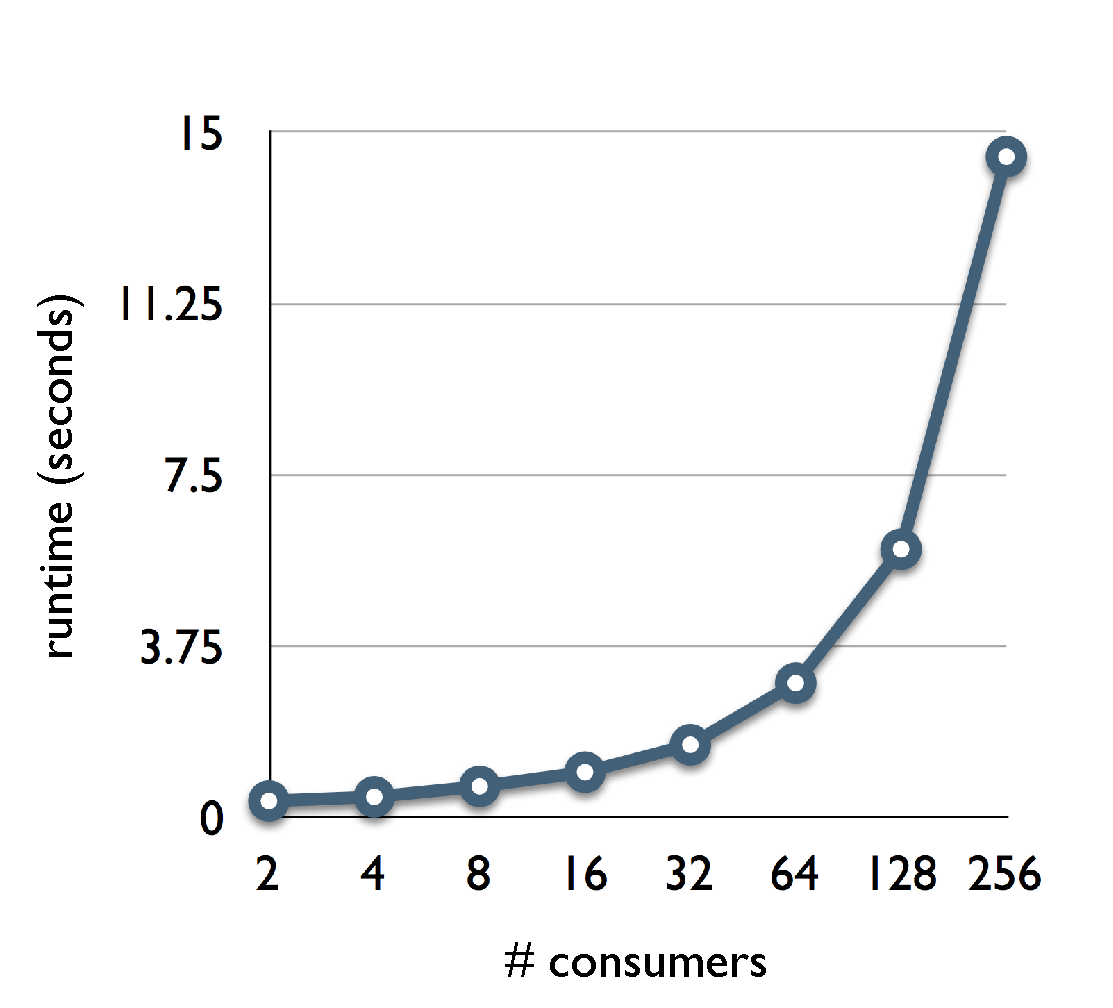
\includegraphics[height=50mm]{fig/sig_exp_rt.eps}
%            \label{fig:fw}
%        \end{figure}
%        \column{0.5\textwidth}
%        \begin{figure}[ht!]
%            \centering
%            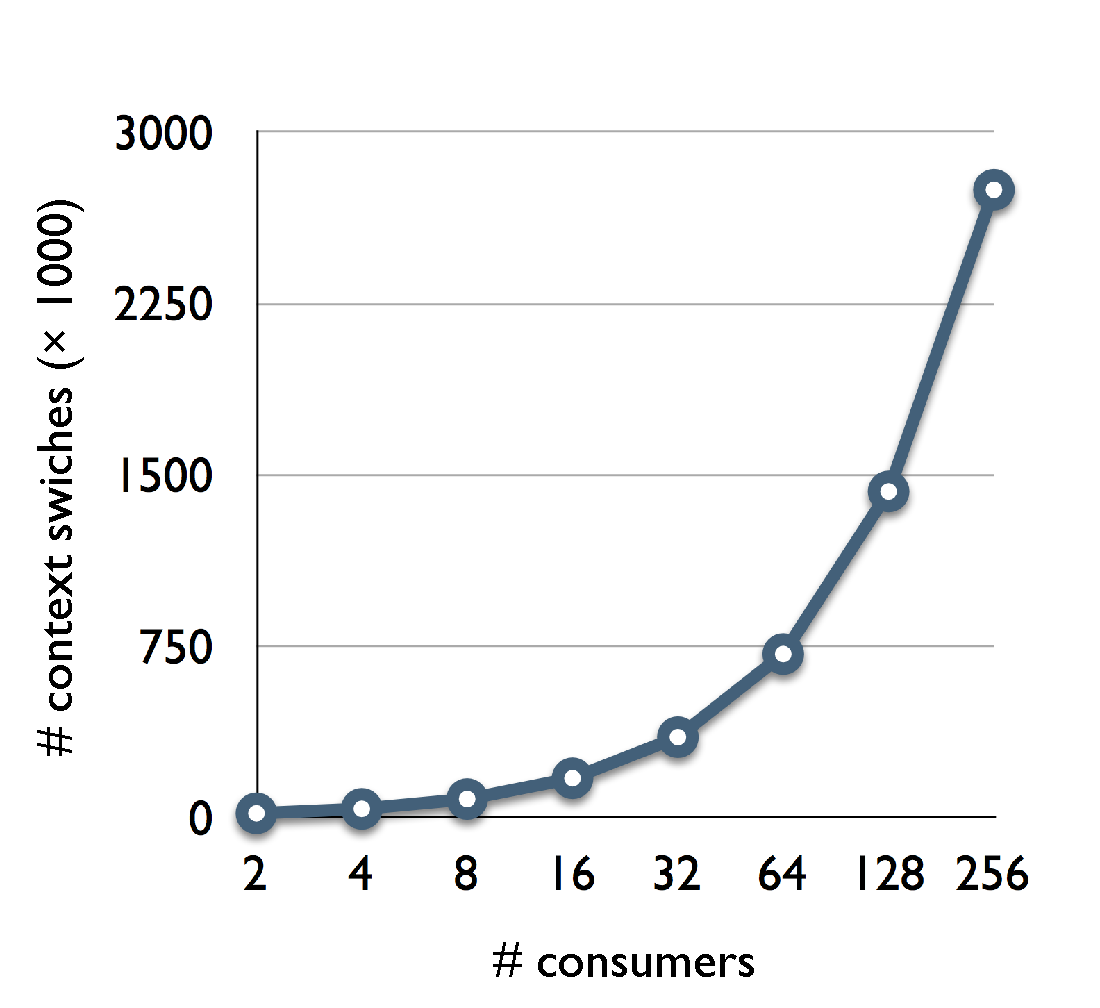
\includegraphics[height=50mm]{fig/sig_exp_cs.eps}
%            \label{fig:fw}
%        \end{figure}
%    \end{columns}
%\end{frame}

%\begin{frame} 
%    \frametitle{Problems We Need to Overcome}
%    \begin{itemize}
%        \item How to evaluate predicates?
%        \item How to automatically signal thread and avoid signallAll?
%        \item How to reduce predicate evaluations? 
%    \end{itemize}
%\end{frame}

\begin{frame}[fragile]
    \frametitle{AutoSynch Framework}
    \begin{figure}[ht!]
        \centering
        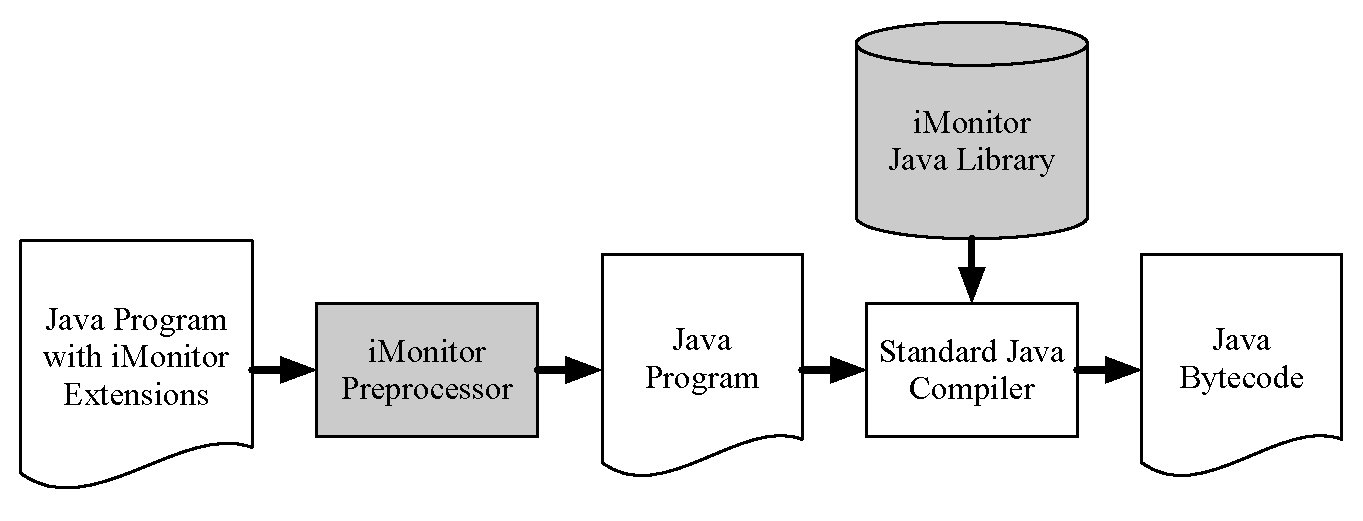
\includegraphics[width=85mm]{fig/flow.eps}
        \label{fig:fw}
    \end{figure}
         
\end{frame}


\section{Our Approach}

\subsection{Evaluate Predicate: Closure}
\begin{frame}
    \frametitle{Closure}
    %The thread owning a monitor performs predicate evaluations for other
    %threads and signaling the appropriated threads before leaving the monitor
    \only<1> {
        \begin{figure}[ht!]
            \centering
            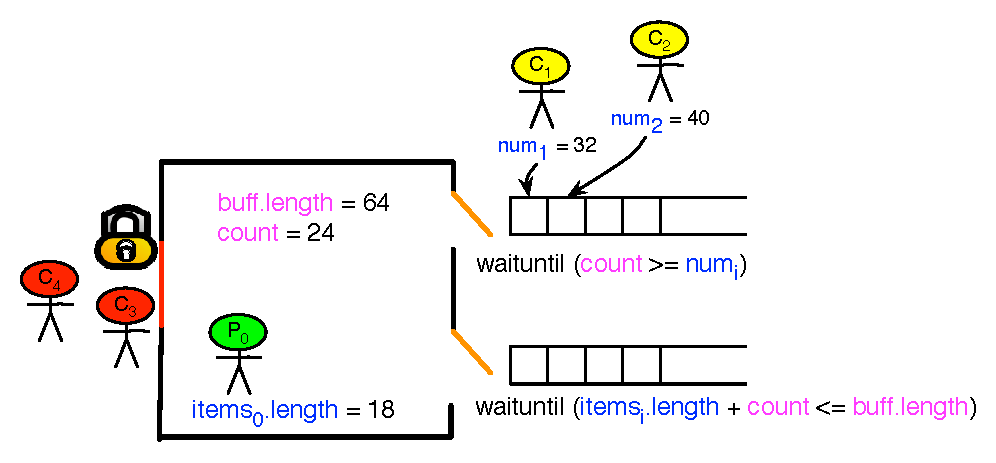
\includegraphics[scale=0.75]{fig/eval_exp_1.eps}
        \end{figure}
    }
    \only<2> {
        \begin{figure}[ht!]
            \centering
            \includegraphics[scale=0.75]{fig/eval_exp_2.eps}
        \end{figure}
    }
    \only<3> {
        \begin{figure}[ht!]
            \centering
            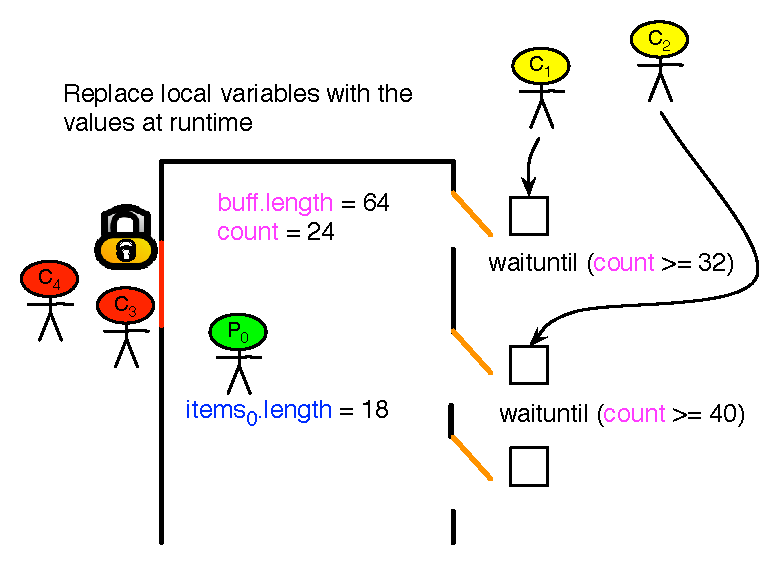
\includegraphics[scale=0.75]{fig/eval_exp_3.eps}
        \end{figure}
    }
    \only<4> {
        \begin{figure}[ht!]
            \centering
            \includegraphics[scale=0.75]{fig/eval_exp_4.eps}
        \end{figure}
    }
\end{frame}


%\begin{frame}[t]
%    \frametitle{Predicate Evaluation}
%    {\bf Observation}: Local variables can be accessed by their owner;
%    therefore, the values of local variables are never changed when their
%    owner are waiting. 
%    \begin{block}{Closure}
%        Given a complex predicate $P(\vec{x}, \vec{a}): X \times A \rightarrow 
%        \mathbb{B}$, where $X \subseteq S$ and $A \subseteq L$. The closure 
%        of $P$ at runtime $t$ is the new shared predicate
%        \[
%        G_t(\vec{x}) = P(\vec{x}, \vec{a_t}),
%        \]
%        where $\vec{a_t}$ is the values of $\vec{a}$ at runtime $t$. 
%    \end{block}
%\end{frame}

\subsection{Avoid signalAll Calls: Relay Signaling Rule}

\begin{frame}
    \frametitle{Relay Signaling Rule}
    \only<1> {
        \begin{figure}[ht!]
            \centering
            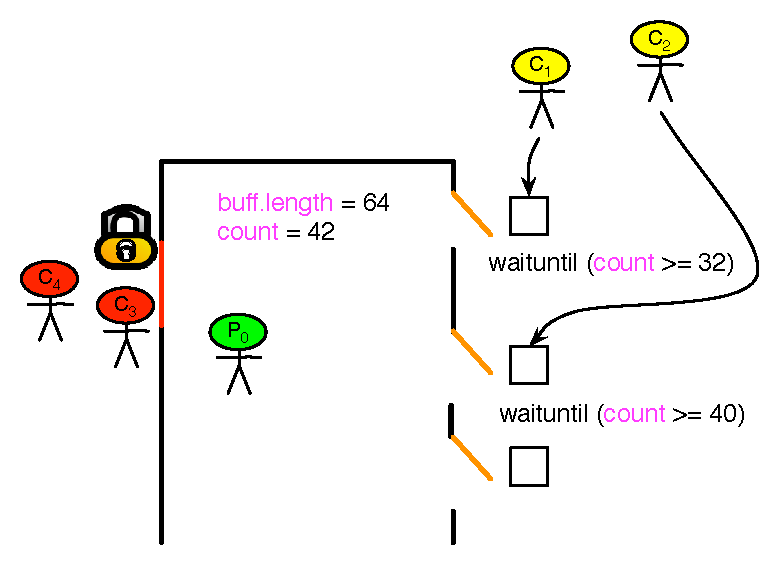
\includegraphics[scale=0.75]{fig/sig_exp_1.eps}
        \end{figure}
    }
    \only<2> {
        \begin{figure}[ht!]
            \centering
            \includegraphics[scale=0.75]{fig/sig_exp_2.eps}
        \end{figure}
    }
    \only<3> {
        \begin{figure}[ht!]
            \centering
            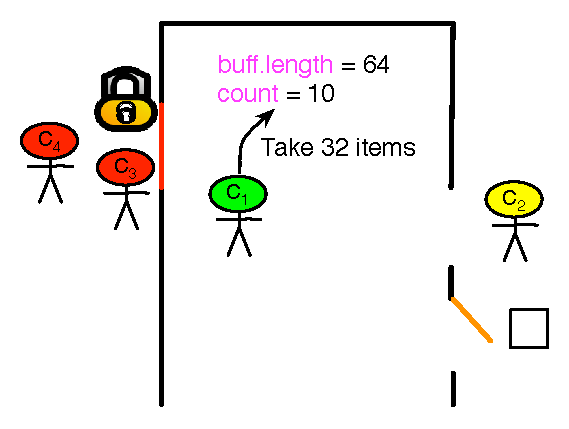
\includegraphics[scale=0.75]{fig/sig_exp_3.eps}
        \end{figure}
    }
    \only<4> {
        \begin{figure}[ht!]
            \centering
            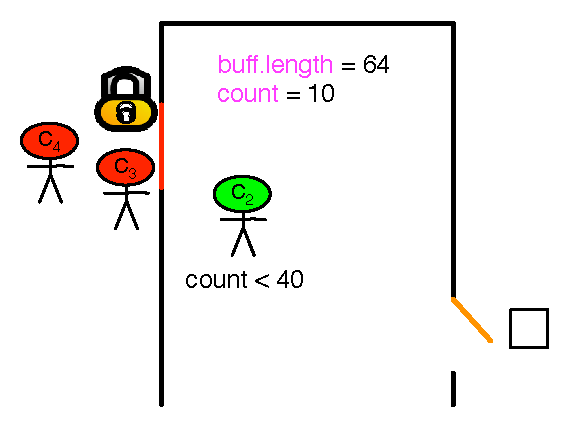
\includegraphics[scale=0.75]{fig/sig_exp_4.eps}
        \end{figure}
    }
    \only<5> {
        \begin{figure}[ht!]
            \centering
            \includegraphics[scale=0.75]{fig/sig_exp_5.eps}
        \end{figure}
    }
\end{frame}

\begin{frame}
    \frametitle{Relay Signaling Rule}
    \begin{itemize}
        \item Before exiting a monitor 
            \pause
        \item Signal {\bf at most one} thread waiting on a condition that 
            has become true
        %    \pause
        %\item If there is one such waiting thread exists, then signals the 
        %    thread
        %    \pause
        %\item The privilege to enter the monitor is transmitted from one thread to 
        %    another thread whose condition has become true
    \end{itemize}
    %\begin{block}{}
    %    Signal {\bf at most one} thread waiting on a predicate that has become
    %    true
    %\end{block}
\end{frame}

\subsection{Reduce Predicate Evaluations: Predicate Tagging}


\begin{frame}
    \frametitle{Predicate Tagging}

    Three types of predicates:
    \begin{enumerate}
    \item Equivalence predicate: $x=5$, $y=a$
    \item Threshold predicate: $x > 8$, $y < b$, $z \ge c + 3$
    \item None of above: $x \ne 3$, $assertion.isTrue()$
    \end{enumerate}
\end{frame}

    
\begin{frame}
    \frametitle{Predicate Tagging}
    \begin{itemize}
        \item Three types of tags: \textcolor{red}{equivalence},
            \textcolor{brown}{threshold}, and \textcolor{blue}{none}
        \item Convert every predicate into disjunctive normal form (DNF)
        \item Assign a tag to every conjunction 
        \item Assignment order: equivalence > threshold > none
        \item e.g. $((x<5) \wedge (y=3)) \vee ((x > 5) \wedge foo1()) \vee
            foo2()$
            \begin{itemize}
                \item \textcolor{red}{$((x < 5) \wedge (y=3))$} 
                \item \textcolor{brown}{$((x > 5) \wedge foo1())$} 
                \item \textcolor{blue}{$foo2()$}
            \end{itemize}
    \end{itemize}
\end{frame}
\begin{frame}
    \frametitle{Predicate Tagging}
    \only<1> {
        \begin{figure}[ht!]
            \centering
            \includegraphics[scale=0.50]{fig/tag_exp_1.eps}
            \label{fig:fw}
        \end{figure}
    }
    \only<2> {
        \begin{figure}[ht!]
            \centering
            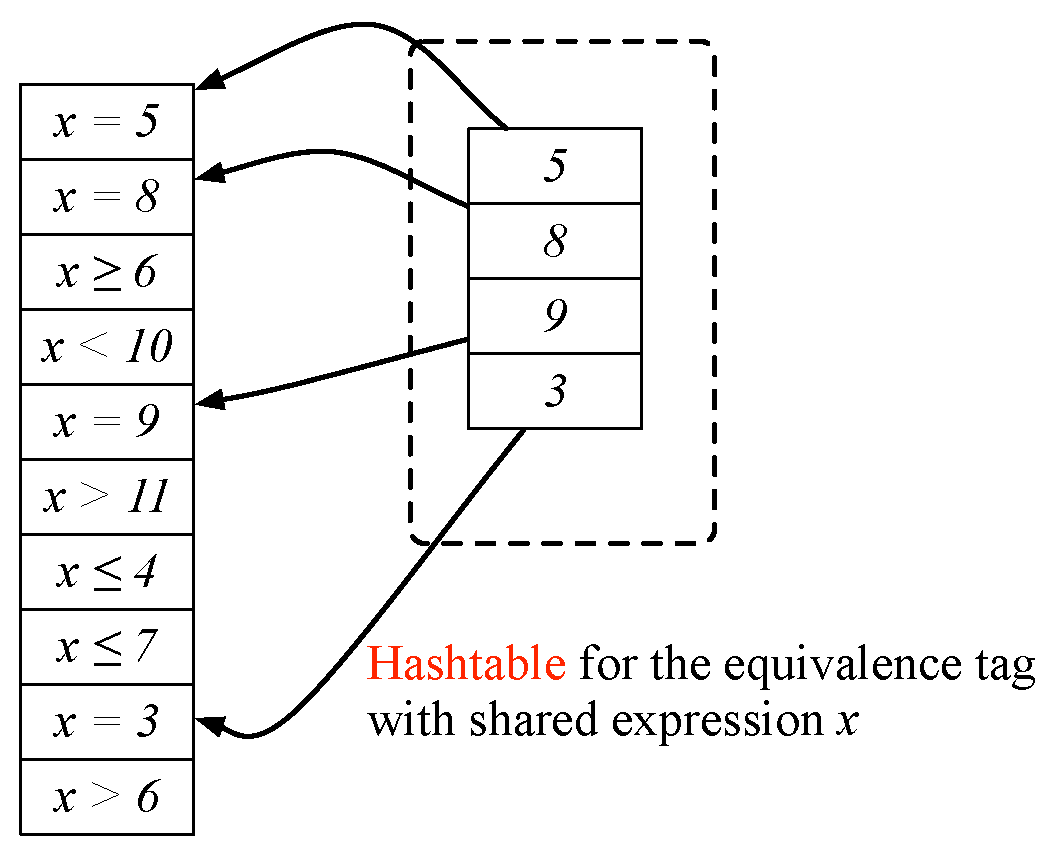
\includegraphics[scale=0.50]{fig/tag_exp_2.eps}
            \label{fig:fw}
        \end{figure}
    }
    \only<3> {
        \begin{figure}[ht!]
            \centering
            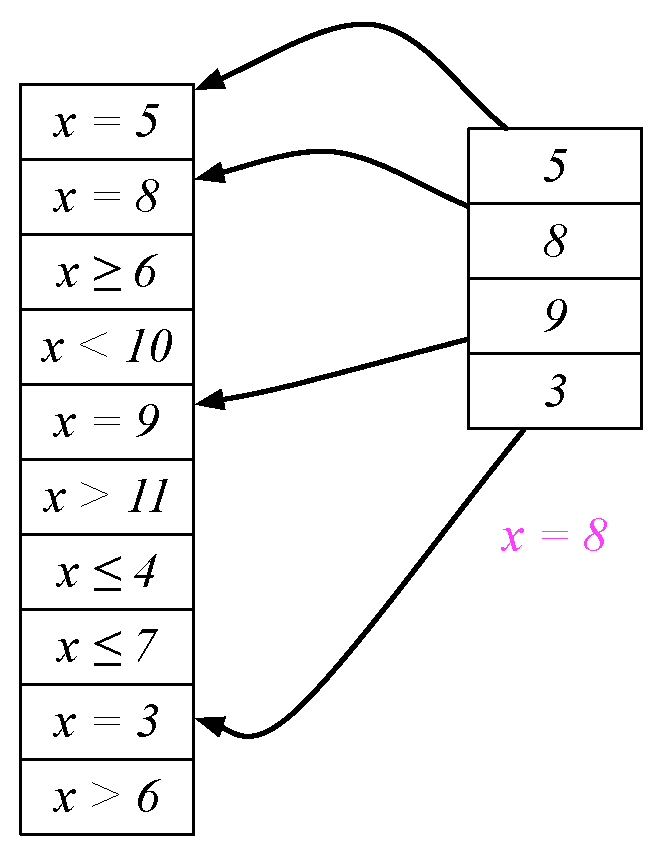
\includegraphics[scale=0.50]{fig/tag_exp_3.eps}
            \label{fig:fw}
        \end{figure}
    }
    \only<4> {
        \begin{figure}[ht!]
            \centering
            \includegraphics[scale=0.50]{fig/tag_exp_4.eps}
            \label{fig:fw}
        \end{figure}
    }
    \only<5> {
        \begin{figure}[ht!]
            \centering
            \includegraphics[scale=0.50]{fig/tag_exp_5.eps}
            \label{fig:fw}
        \end{figure}
    }
    \only<6> {
        \begin{figure}[ht!]
            \centering
            \includegraphics[scale=0.50]{fig/tag_exp_6.eps}
            \label{fig:fw}
        \end{figure}
    }
    \only<7> {
        \begin{figure}[ht!]
            \centering
            \includegraphics[scale=0.50]{fig/tag_exp_7.eps}
            \label{fig:fw}
        \end{figure}
    }
    \only<8> {
        \begin{figure}[ht!]
            \centering
            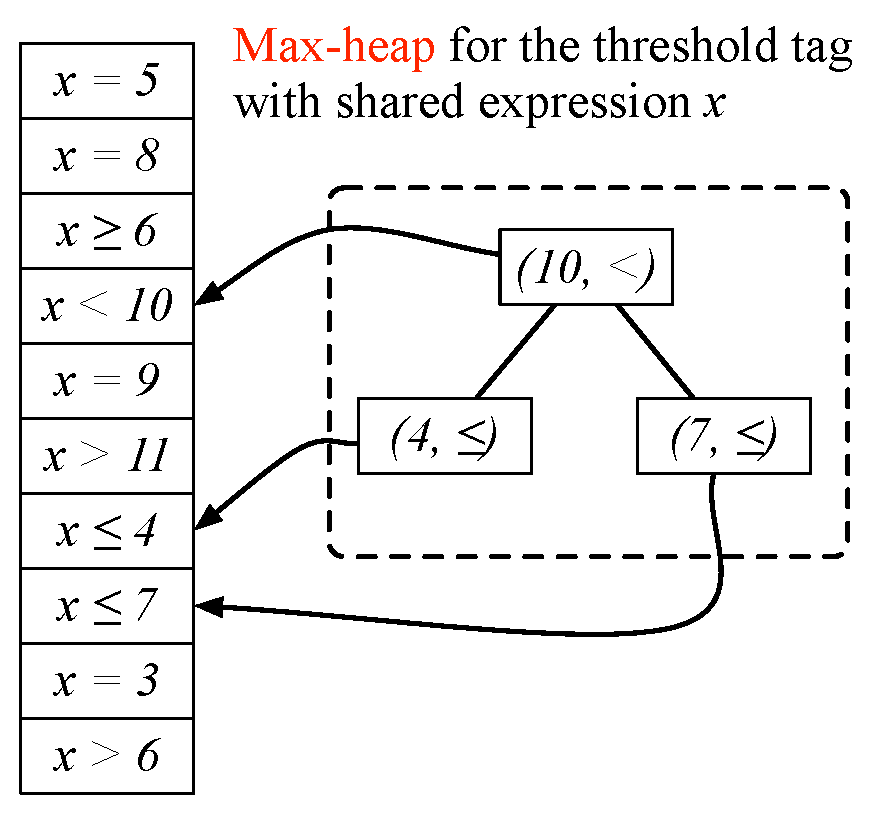
\includegraphics[scale=0.50]{fig/tag_exp_8.eps}
            \label{fig:fw}
        \end{figure}
    }
\end{frame}

\section{Results}

\begin{frame}
    \frametitle{Evaluation}
    Four different signaling approaches: 
    \begin{description}[labelwidth=0]
        \item[Explicit] Using the Java explicit-signal 
        \item[Baseline] Automatic-signal relying on only one condition variable. 
        \item[AutoSynch-T] Using closure and relay signaling rule but predicate 
            tagging
        \item [AutoSynch] Using closure, relay signaling rule and predicate
            tagging
    \end{description}
\end{frame} 

\begin{frame}
    \frametitle{Evaluation}
    %Two types of evaluations
    %\begin{description}
    %    \item[Saturation] Only performing monitor accessing functions 
    %    \item[Work load] Performing other operations out of the monitor between
    %        every two monitor operations
    %\end{description}
    Three types of problems:
    \begin{description}[labelwidth=\widthof{Complex}]
        \item[Shared predicate] Depends only on shared variables
            \begin{itemize}
                \item bounded-buffer, $H_2O$ problem  
            \end{itemize}
        \item[Complex predicate] Depends on both shared and local variables 
            \begin{itemize}
                \item readers-writers, round-robin access pattern
            \end{itemize}
        \item[signalAll] Requires signalAll calls
            \begin{itemize}
                \item parameterized bounded-buffer
            \end{itemize}
    \end{description}
\end{frame}

\begin{frame}
    \frametitle{Evaluation: Shared Predicate}
    \begin{columns}[c]
        \column{0.5\textwidth}
            \begin{figure}[ht!]
                \centering
                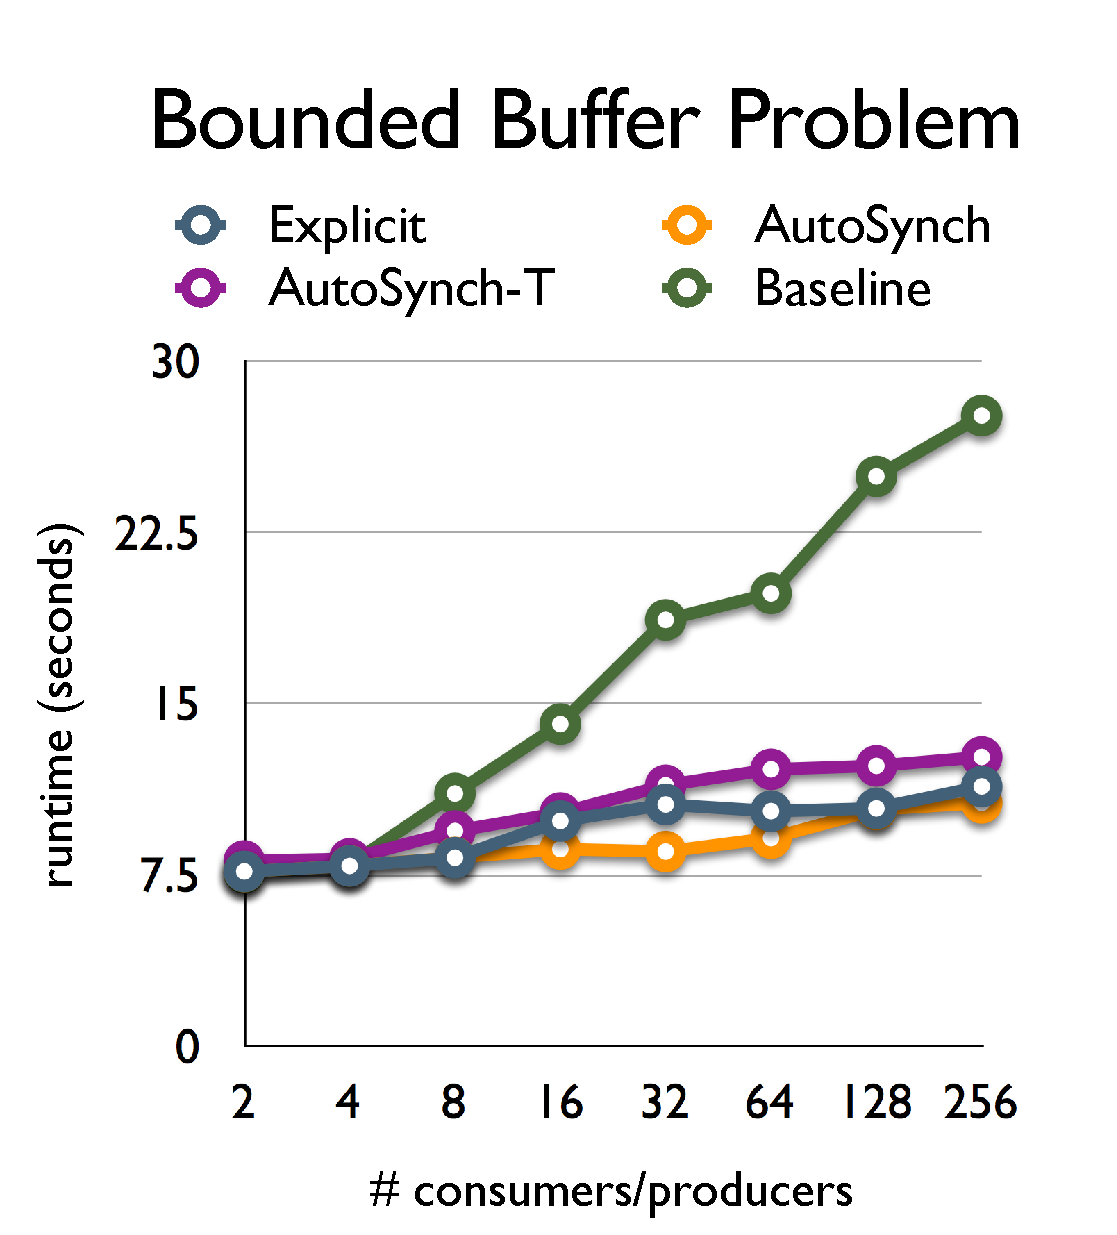
\includegraphics[width=56mm]{fig/pc.eps}
                \label{fig:pc_eval}
            \end{figure}
        \column{0.5\textwidth}
       % \pause
            \begin{figure}[ht!]
                \centering
                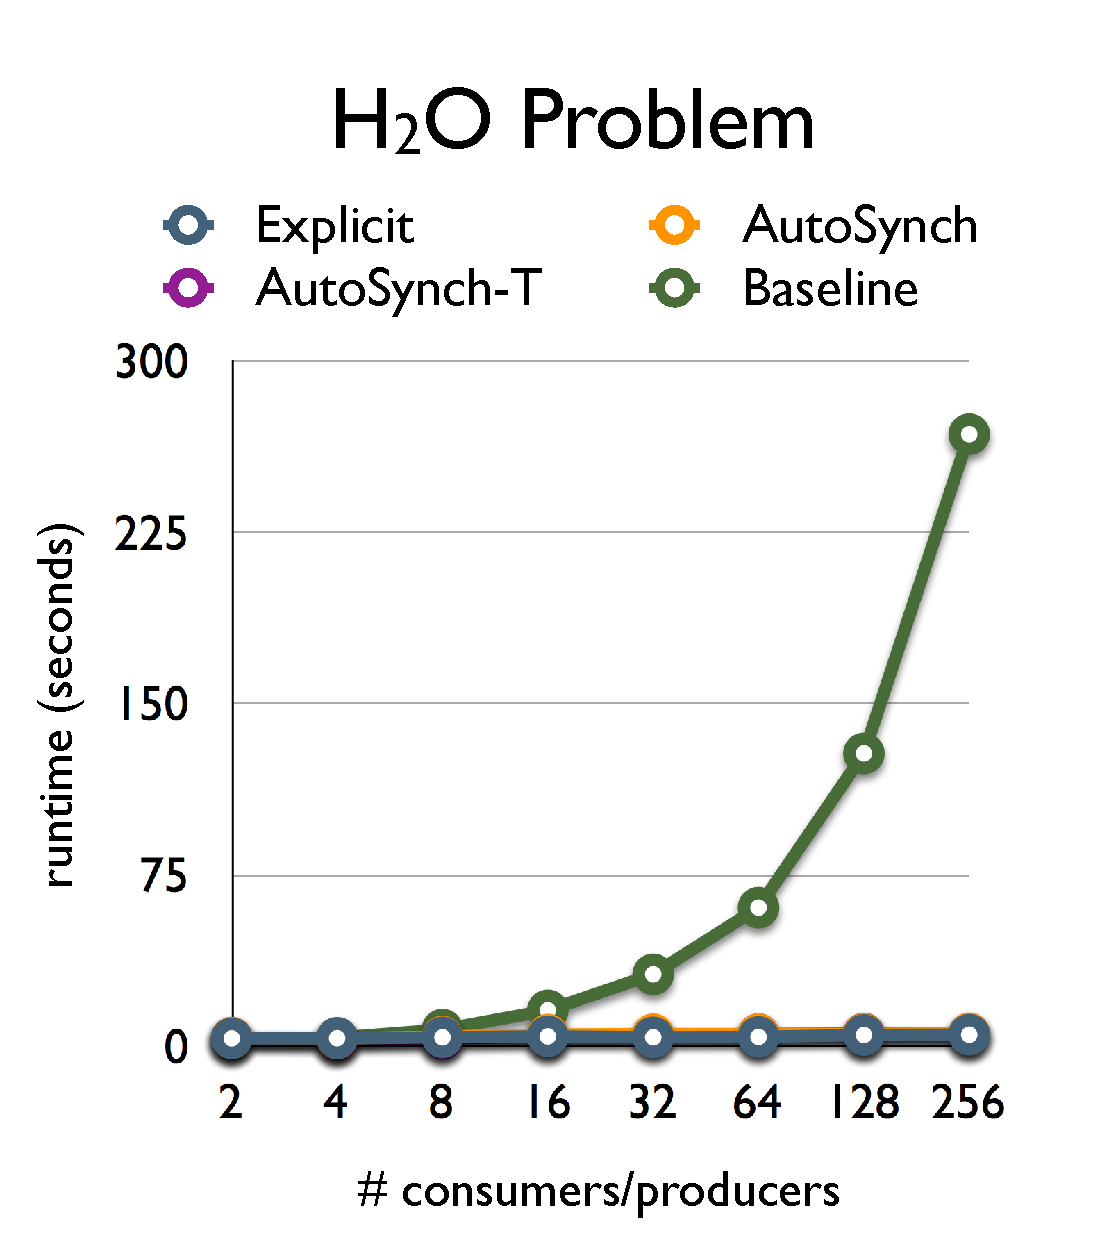
\includegraphics[width=56mm]{fig/h2o.eps}
                \label{fig:h2o_eval}
            \end{figure}
    \end{columns}
\end{frame}

\begin{frame}[t]
    \frametitle{Evaluation: Complex Predicate}
    \begin{columns}
        \column{0.5\textwidth}
        \begin{figure}[ht!]
            \centering
            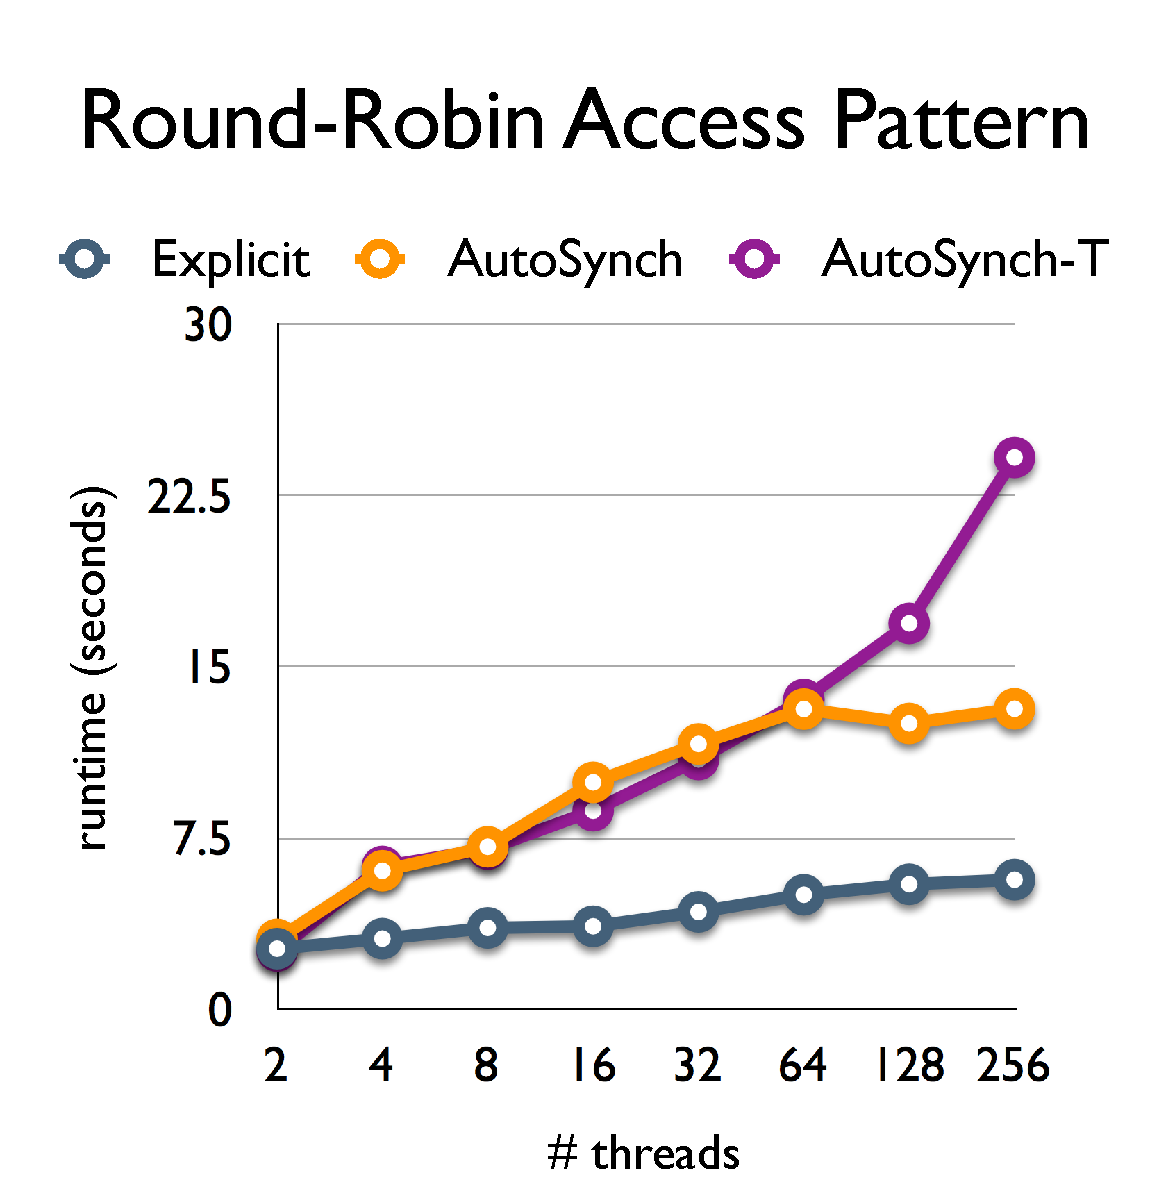
\includegraphics[width=56mm]{fig/rr.eps}
            \label{fig:rr_eval}
        \end{figure}
        \column{0.5\textwidth}
       % \pause
        \begin{figure}[ht!]
            \centering
            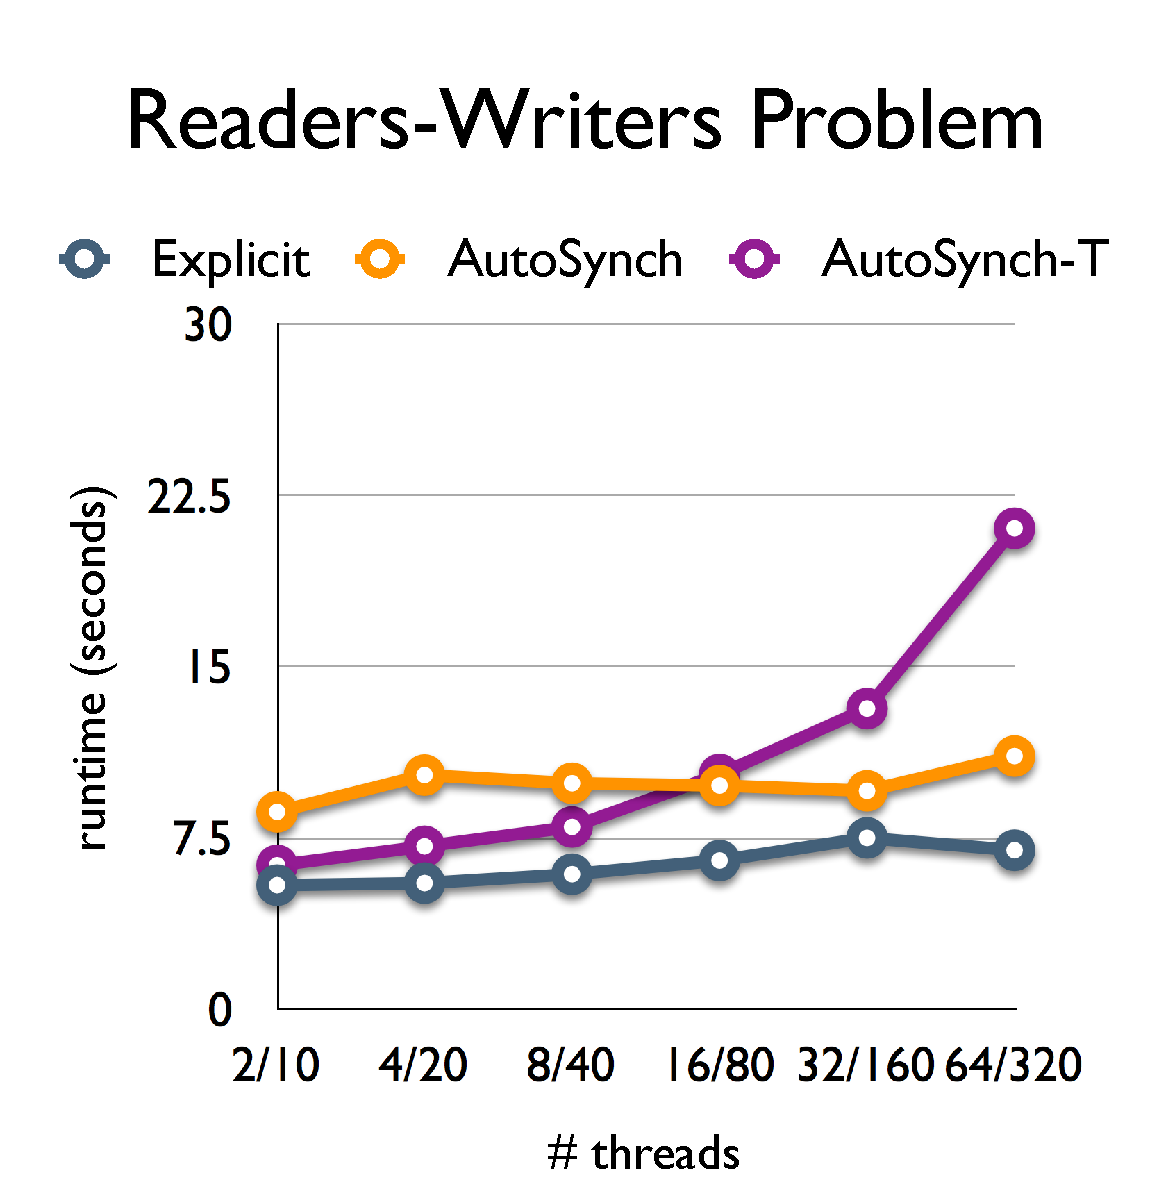
\includegraphics[width=56mm]{fig/trw.eps}
            \label{fig:rw_eval}
        \end{figure}
    \end{columns}
\end{frame}

\begin{frame}
    \frametitle{Evaluation: signalAll}
    \textcolor{black}{Parameterized Bounded Buffer (Requires signalAll calls)}
    \begin{columns}[c]
        \column{0.5\textwidth}
            \begin{figure}[ht!]
                \centering
                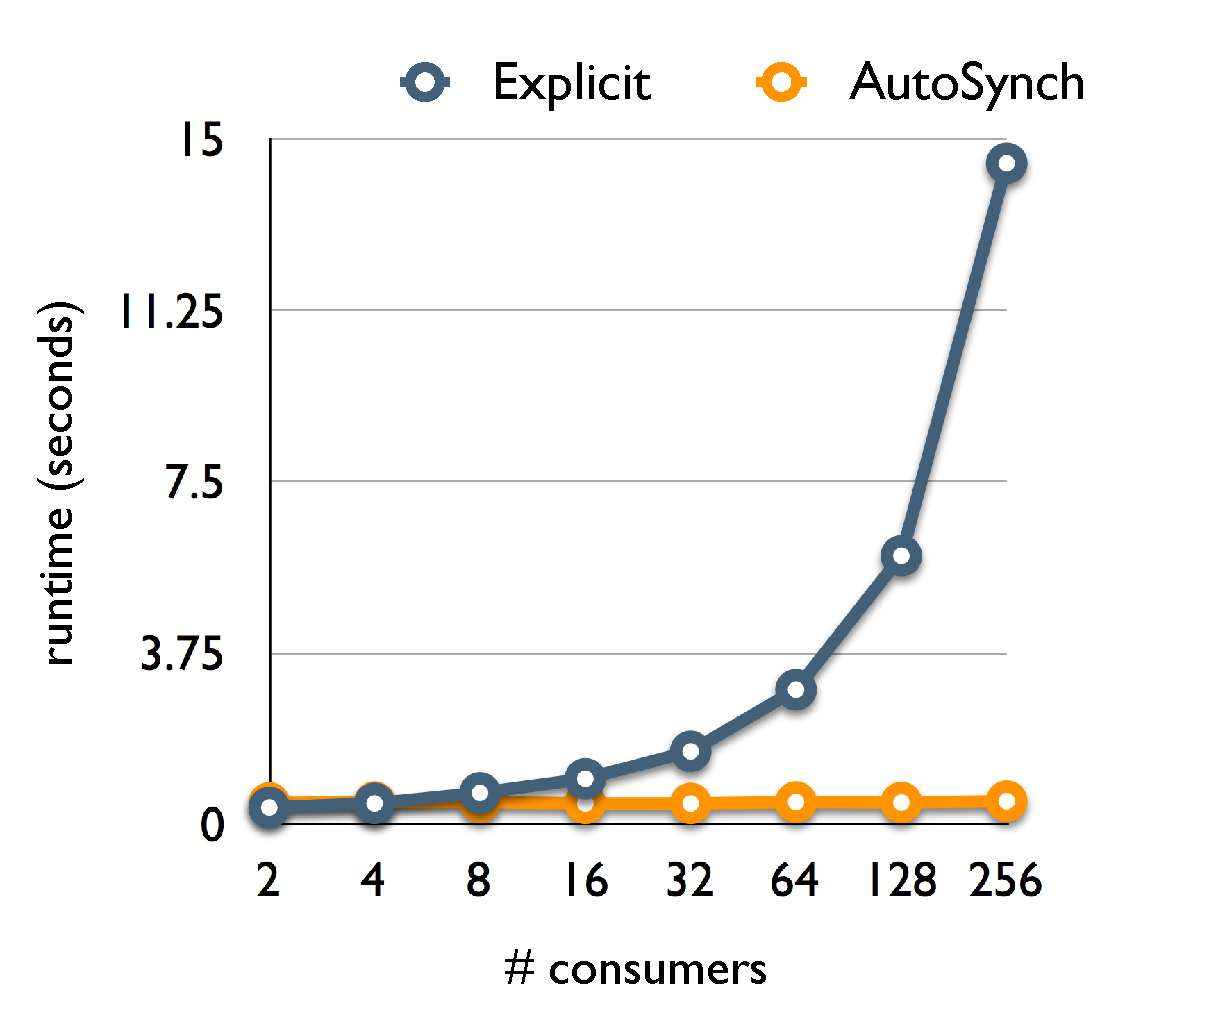
\includegraphics[width=56mm]{fig/rpc.eps}
                \label{fig:rpc_eval}
            \end{figure}
        \column{0.5\textwidth}
            \begin{figure}[ht!]
                \centering
                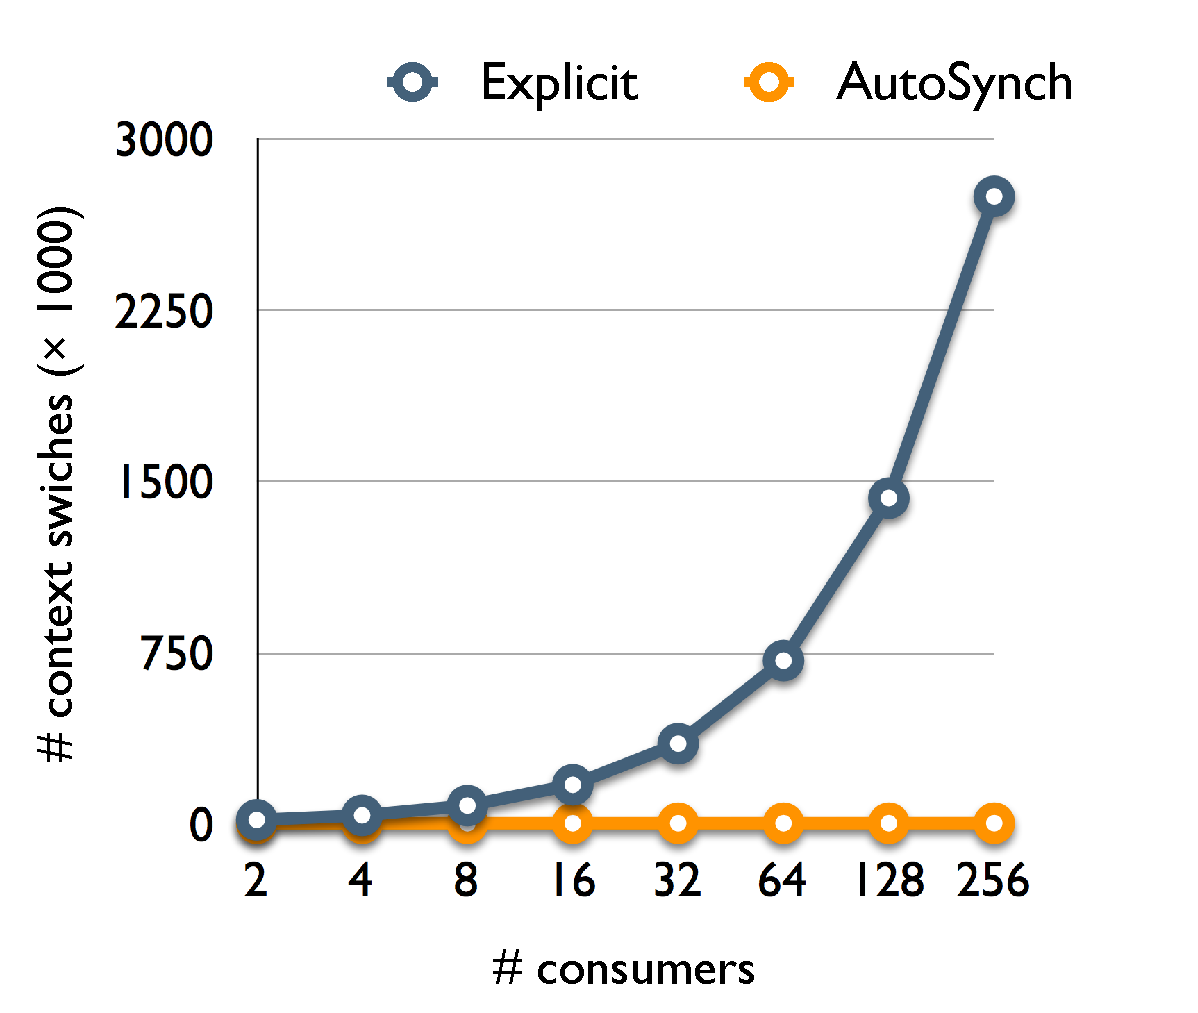
\includegraphics[width=56mm]{fig/csrpc.eps}
            \label{fig:csrpc_eval}
            \end{figure}
    \end{columns}
\end{frame}

\begin{frame}
    \frametitle{Evaluation: Workload}
    Workload Simulation
    \begin{itemize}
        \item Evaluate performance of AutoSynch under different workloads
        \item Perform other operations out of the monitor between every two monitor
            operations
        \item Report runtime ratio with respect to Explicit
    \end{itemize}
\end{frame}

\begin{frame}
    \frametitle{Evaluation: Workload}
    \begin{columns}[c]
        \column{0.5\textwidth}
        \begin{figure}[ht!]
            \centering~
            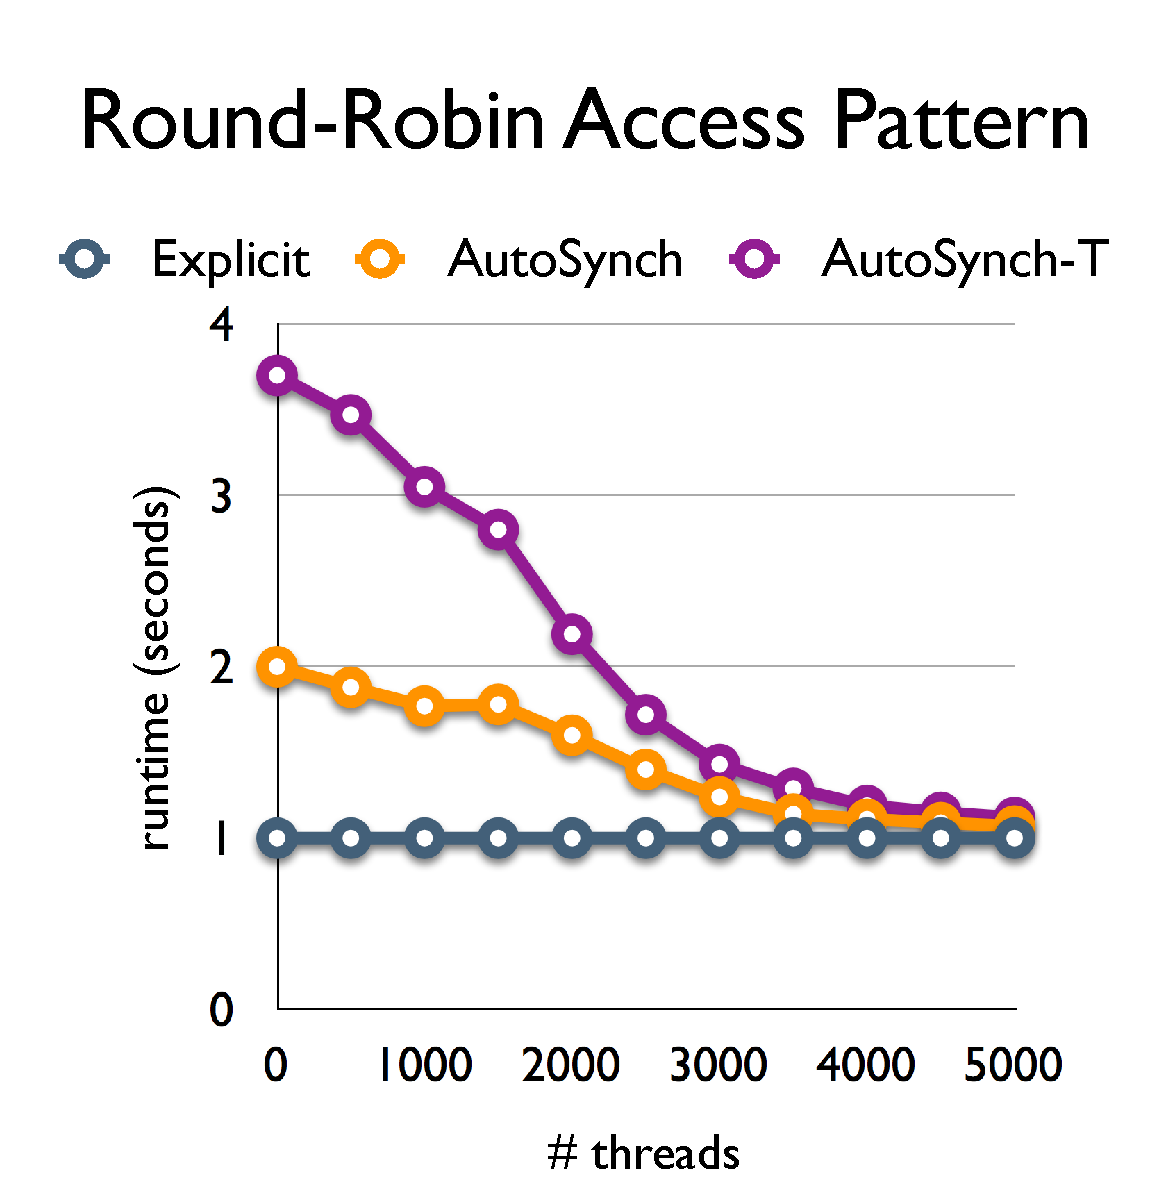
\includegraphics[width=56mm]{fig/srr.eps}
        \label{fig:rr_ratio}
        \end{figure}

        %\pause
        \column{0.5\textwidth}
        \begin{figure}[ht!]                                                             
            \centering                                                                    
            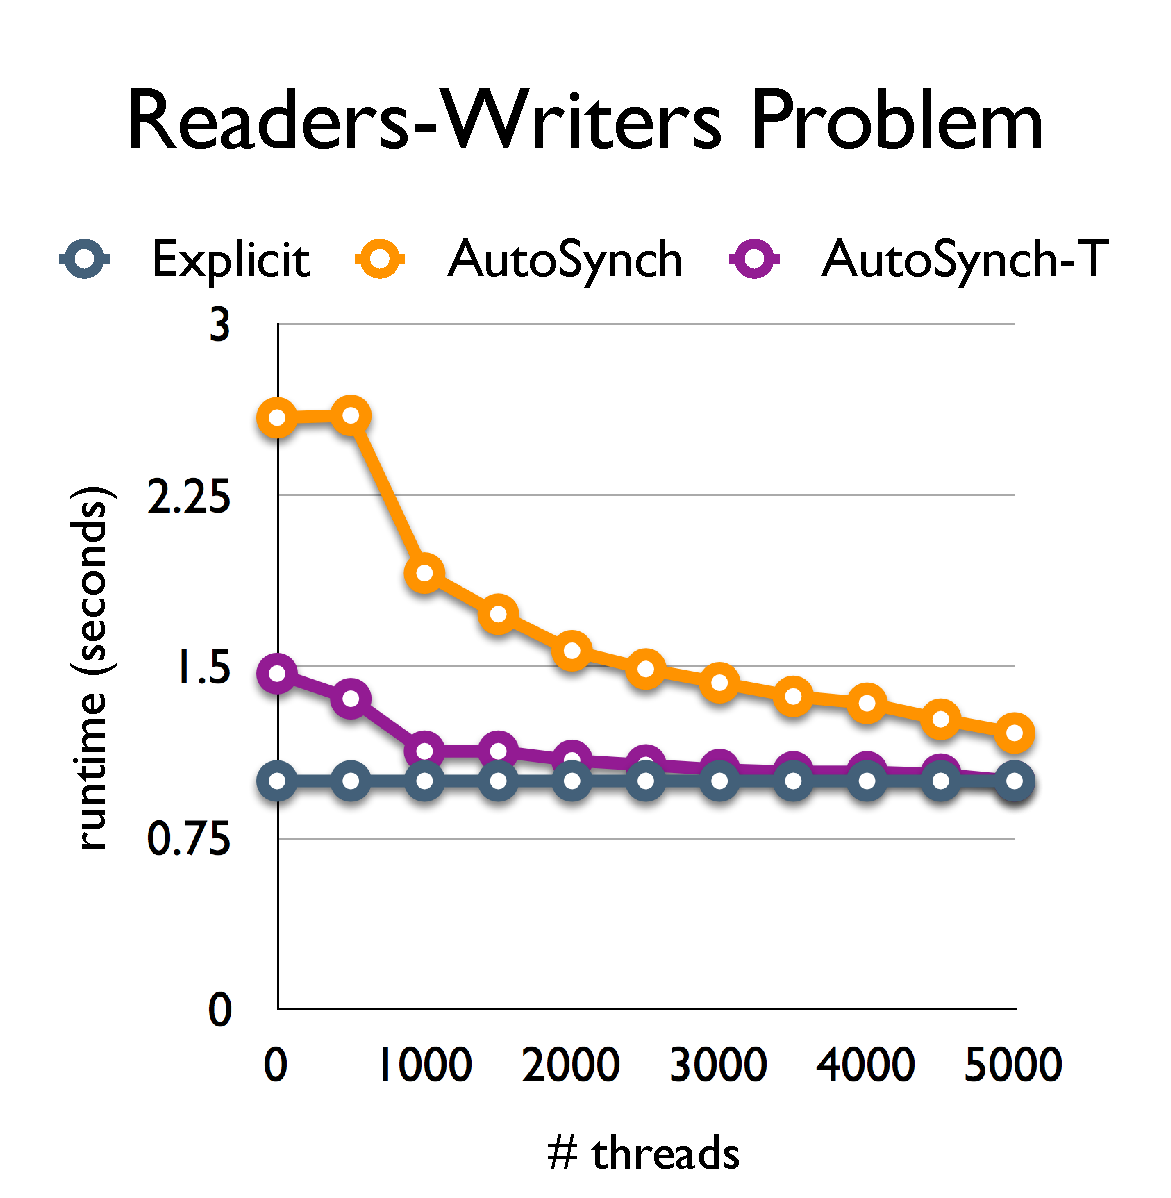
\includegraphics[width=56mm]{fig/strw.eps}                                    
        \label{fig:trw_ratio}                                                           
        \end{figure}
    \end{columns}
\end{frame}

\section{Conclusions and Future Work}

\begin{frame}
    \frametitle{Conclusions and Future Work}
    Conclusions
    \begin{itemize}
        %\item Introducing {\em closure} that enables the predicate evaluation in
        %    every thread
        %\item Using {\em relay signal invariance} to avoid signalAll calls
        %\item Investigating {\em predicate tag} to efficiently determine a
        %    thread that should be signaled 
        \item We propose AutoSynch that supports automatic signaling with
            simple syntax
        \item AutoSynch is almost as efficient as
            the explicit-signal or even more efficient
    \end{itemize}
    Future work
    \begin{itemize}
%        \item Fairness is not guaranteed
        \item Use the architecture information
        \item Implement AutoSynch directly in JVM 
%        \item Implementing in other programming languages
%        \item Comparing with other transactional memory approaches
%        \item More practical applications 
    \end{itemize}

\end{frame}


%\begin{frame}[t]
%\frametitle{Motivation}
%\end{frame}

\end{document}
